\documentclass[conference,11pt]{IEEEtran}

\usepackage[utf8]{inputenc}
\usepackage[T1]{fontenc}
\usepackage{amsmath,amssymb}
\usepackage{graphicx}
\usepackage{booktabs}
\usepackage{algorithm}
\usepackage{algpseudocode}
\usepackage{listings}
\usepackage{xcolor}
\usepackage{hyperref}
\usepackage{multirow}
\usepackage{tikz}
\usetikzlibrary{arrows.meta,positioning,shapes.geometric,fit}
\usepackage{subcaption}
\usepackage{balance}

\definecolor{codebg}{rgb}{0.96,0.96,0.96}
\definecolor{codegreen}{rgb}{0.0,0.5,0.0}
\definecolor{codegray}{rgb}{0.5,0.5,0.5}
\definecolor{codepurple}{rgb}{0.58,0.0,0.82}

\lstset{
  backgroundcolor=\color{codebg},
  basicstyle=\ttfamily\footnotesize,
  breaklines=true,
  captionpos=b,
  commentstyle=\color{codegreen},
  keywordstyle=\color{codepurple}\bfseries,
  stringstyle=\color{red},
  numberstyle=\tiny\color{codegray},
  numbers=left,
  frame=single,
  tabsize=2,
  showstringspaces=false
}

\lstdefinelanguage{TypeScript}{
  keywords={class, interface, type, function, const, let, var, return, if, else, for, while, switch, case, break, continue, new, this, extends, implements, export, import, from, async, await, readonly, enum, null, undefined, true, false, typeof, instanceof},
  sensitive=true,
  comment=[l]{//},
  morecomment=[s]{/*}{*/},
  morestring=[b]',
  morestring=[b]"
}

\title{BlackSwan: Recursive Self-Improvement of a Java Decompiler\\via AI-Driven Code Modification and\\Multi-Metric Evaluation}

\author{
\IEEEauthorblockN{Ghast}
\IEEEauthorblockA{BlackSwan\\
\url{https://www.blackswan.sh}}
}

\begin{document}

\maketitle

\begin{abstract}
We present BlackSwan, a Java bytecode decompiler implemented in TypeScript that improves itself through a recursive feedback loop driven by an AI coding agent (Claude Code). The system comprises five layers: a complete port of the OW2 ASM bytecode manipulation library to TypeScript (${\sim}12{,}000$ lines), a typed intermediate representation with 19 expression and 13 statement node types organized into control flow graphs, an analysis framework supporting class hierarchy construction, virtual method table resolution, and dataflow-driven optimization passes, a multi-strategy decompiler with structured control flow recovery and fallback emission, and an AI post-processor for runtime output cleanup. We evaluate decompiler output against original source code using a composite metric drawn from nine similarity measures spanning textual, sequential, compression-based, and structural categories. In the recursive loop, the AI agent reads benchmark scores, reads the decompiler's own source code alongside competing decompilers' output, and proposes targeted patches. After iterative self-improvement, BlackSwan achieves a composite similarity score of 0.8693 on a 47-class benchmark, within 0.7\% of CFR (0.8760), a decompiler with over a decade of manual development. We discuss implications for automated deobfuscation, where the loop can be specialized against known obfuscation tools by providing obfuscator source code and paired samples.
\end{abstract}

\begin{IEEEkeywords}
decompilation, reverse engineering, self-improving systems, large language models, intermediate representation, Java bytecode, program analysis
\end{IEEEkeywords}

%% ============================================================
\section{Introduction}
\label{sec:intro}

Java bytecode decompilation---the recovery of human-readable source code from compiled \texttt{.class} files---has been an active area of research and tooling for over two decades. Existing production decompilers such as CFR~\cite{cfr}, Procyon~\cite{procyon}, Vineflower~\cite{vineflower}, and FernFlower~\cite{fernflower} are predominantly maintained by small teams or individual developers. Each exhibits distinct strengths and failure modes: CFR excels at control flow recovery but may mangle variable naming, Procyon handles generics faithfully but struggles with certain obfuscated switch patterns, and Vineflower produces clean output on standard code but encounters difficulties with edge cases in exception handling.

A fundamental asymmetry exists in the obfuscation-decompilation arms race. Obfuscation is \emph{mechanical}: applying a transformation at build time requires implementing a single pass. Decompilation is \emph{analytical}: reversing that transformation requires understanding its structure, recognizing its patterns in arbitrary contexts, and generating correct inverse operations. A single developer can add a new obfuscation pass in a weekend; adapting all existing decompilers to handle it may take months.

We propose a fundamentally different approach: rather than manually engineering decompilation heuristics, we construct a decompiler whose source code can be iteratively modified by an AI coding agent in a closed feedback loop. The agent reads benchmark scores comparing the decompiler's output against ground truth, reads the decompiler's own source, reads competing decompilers' output on the same inputs, and proposes targeted patches. The benchmark is re-run and the loop continues.

This approach required a significant engineering investment: the entire decompilation pipeline---from bytecode parsing to source emission---was implemented in TypeScript rather than Java, because the AI agent (Claude Code) exhibits substantially stronger code comprehension and editing capabilities in TypeScript. The resulting system, BlackSwan, comprises approximately 32,000 lines of TypeScript across five packages.

Our contributions are:
\begin{enumerate}
    \item A complete TypeScript port of OW2 ASM~\cite{asm}, supporting Java class file versions 45.3 through 65.0 (Java 1.1--21).
    \item A typed intermediate representation inspired by MapleIR~\cite{mapleir} with 19 expression types, 13 statement types, and a stack-simulating IR builder.
    \item A multi-metric evaluation framework using nine similarity measures with weighted composite scoring, designed to resist Goodhart's Law~\cite{goodhart} under optimization pressure.
    \item Empirical demonstration that recursive AI-driven code modification produces measurable, persistent improvements in decompiler output quality.
    \item A discussion of applications to automated deobfuscation via obfuscator-specialized decompiler variants.
\end{enumerate}

%% ============================================================
\section{Related Work}
\label{sec:related}

\subsection{Java Decompilation}

Modern Java decompilers share a common architecture: bytecode parsing, intermediate representation construction, control flow analysis, type inference, and source emission. FernFlower~\cite{fernflower}, the IntelliJ IDEA default, uses an SSA-based IR with iterative dataflow analysis. CFR~\cite{cfr} employs aggressive pattern matching for control flow reconstruction. Procyon~\cite{procyon} introduced improved generic type recovery. Vineflower~\cite{vineflower}, a FernFlower fork, focuses on output readability through enhanced formatting and variable naming.

All four are written in Java, limiting their accessibility to AI-driven modification pipelines that operate most effectively on dynamically-typed or TypeScript codebases.

\subsection{AI-Assisted Decompilation}

Recent work has explored using large language models (LLMs) directly for decompilation. LLM4Decompile~\cite{llm4decompile} fine-tunes models on paired assembly-source datasets. SLaDe~\cite{slade} uses sequence-to-sequence models for C decompilation. Nova~\cite{nova} applies LLMs to binary code analysis broadly.

These approaches use the LLM as the decompiler itself---performing inference-time translation from low-level to high-level representations. BlackSwan takes a fundamentally different approach: the LLM modifies the \emph{decompiler's source code}, producing persistent improvements that apply to all future inputs without additional inference cost.

\subsection{Self-Improving Systems}

The concept of recursive self-improvement has been explored in program synthesis~\cite{levin2013, schmidhuber2003} and more recently in LLM-driven code generation~\cite{chen2024selfplay, shinn2023reflexion}. Reflexion~\cite{shinn2023reflexion} uses verbal feedback for iterative improvement but operates at inference time. AlphaCode~\cite{alphacode} generates and filters solutions but does not modify its own implementation. BlackSwan is distinguished by targeting the \emph{tool itself} for modification rather than individual outputs.

%% ============================================================
\section{System Architecture}
\label{sec:architecture}

BlackSwan is organized as a monorepo containing five core packages and two applications, with dependencies flowing upward through the stack (Figure~\ref{fig:architecture}).

\begin{figure}[t]
\centering
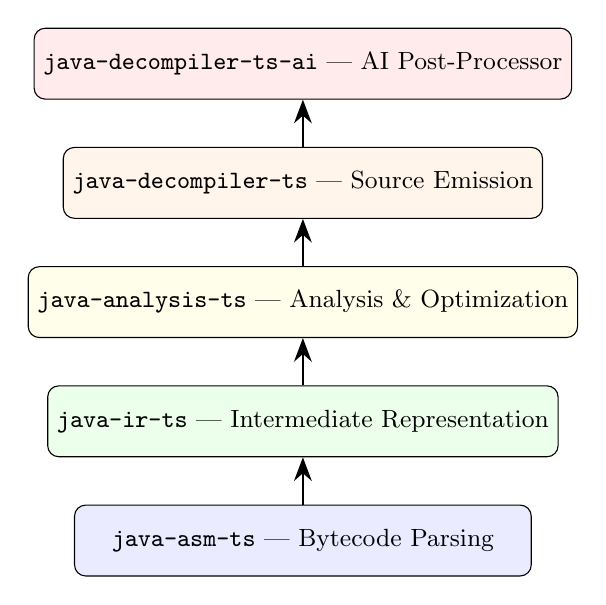
\begin{tikzpicture}[
    box/.style={draw, rounded corners, minimum width=5.8cm, minimum height=0.9cm, align=center, font=\small},
    arr/.style={-{Stealth[length=3mm]}, thick},
    node distance=0.6cm
]
\node[box, fill=blue!8] (asm) {\texttt{java-asm-ts} --- Bytecode Parsing};
\node[box, fill=green!8, above=of asm] (ir) {\texttt{java-ir-ts} --- Intermediate Representation};
\node[box, fill=yellow!8, above=of ir] (analysis) {\texttt{java-analysis-ts} --- Analysis \& Optimization};
\node[box, fill=orange!8, above=of analysis] (decompiler) {\texttt{java-decompiler-ts} --- Source Emission};
\node[box, fill=red!8, above=of decompiler] (ai) {\texttt{java-decompiler-ts-ai} --- AI Post-Processor};

\draw[arr] (asm) -- (ir);
\draw[arr] (ir) -- (analysis);
\draw[arr] (analysis) -- (decompiler);
\draw[arr] (decompiler) -- (ai);
\end{tikzpicture}
\caption{BlackSwan package dependency stack. Each layer depends only on layers below it. All layers are implemented in TypeScript, enabling AI-driven modification at every level.}
\label{fig:architecture}
\end{figure}

\subsection{Design Rationale: TypeScript}

The choice of TypeScript as the implementation language was driven by a single constraint: the recursive improvement loop requires the AI agent to read, comprehend, and edit the decompiler source code. Empirically, Claude Code demonstrates substantially stronger performance on TypeScript code than on equivalent Java implementations, particularly for:

\begin{itemize}
    \item Understanding visitor-pattern architectures with multiple dispatch
    \item Reasoning about bytecode-level operations expressed as typed objects
    \item Proposing correct modifications to control flow reconstruction algorithms
\end{itemize}

This decision required porting the OW2 ASM library---approximately 12,000 lines of mature Java code---to TypeScript, an investment that proved critical to the loop's effectiveness.

%% ============================================================
\section{Bytecode Parsing: ASM Port}
\label{sec:asm}

The \texttt{java-asm-ts} package is a faithful TypeScript port of OW2 ASM~\cite{asm}, preserving its visitor-pattern API and supporting the full JVM class file specification.

\subsection{Scope}

The port supports:
\begin{itemize}
    \item All 200+ JVM opcodes including \texttt{invokedynamic}
    \item Class file format versions 45.3 (Java 1.1) through 65.0 (Java 21)
    \item Complete constant pool parsing (17 constant types)
    \item \texttt{StackMapTable} attribute processing (6 frame types: \texttt{F\_FULL}, \texttt{F\_SAME}, \texttt{F\_SAME1}, \texttt{F\_APPEND}, \texttt{F\_CHOP}, \texttt{F\_NEW})
    \item Generic signature parsing and writing via \texttt{SignatureVisitor}
    \item Module descriptors (Java 9+) and record components (Java 16+)
    \item Bootstrap method attributes for \texttt{invokedynamic}
    \item All access flags (22 distinct flags across class, method, and field contexts)
\end{itemize}

\subsection{Visitor Architecture}

The port preserves ASM's visitor chain pattern:

\begin{lstlisting}[language=TypeScript, caption=Visitor pattern for class traversal]
class ClassVisitor {
  visit(version, access, name, signature,
        superName, interfaces): void
  visitField(access, name, descriptor,
             signature, value): FieldVisitor
  visitMethod(access, name, descriptor,
              signature, exceptions): MethodVisitor
}
\end{lstlisting}

\texttt{ClassReader} performs bottom-up parsing of the binary class file format, dispatching to the appropriate visitor methods. \texttt{ClassWriter} implements the same visitor interface for top-down class file generation, enabling round-trip processing.

\subsection{Validation}

Round-trip correctness is verified: for a given \texttt{.class} file, reading it with \texttt{ClassReader} into a \texttt{ClassWriter} and comparing the emitted bytes against the original input produces identical results. This was used as the convergence criterion during the AI-driven porting process---Claude Code iterated until round-trip tests passed on three reference JAR files.

%% ============================================================
\section{Intermediate Representation}
\label{sec:ir}

The \texttt{java-ir-ts} package defines a typed intermediate representation that lifts the JVM's stack-based instruction set into expression trees organized within a control flow graph.

\subsection{Expression Hierarchy}

The IR defines 19 expression node types (Table~\ref{tab:expressions}), each carrying explicit \texttt{Type} information derived from the ASM type system.

\begin{table}[t]
\centering
\caption{IR Expression Node Types}
\label{tab:expressions}
\footnotesize
\begin{tabular}{@{}ll@{}}
\toprule
\textbf{Category} & \textbf{Types} \\
\midrule
Arithmetic/Logic & \texttt{ArithmeticExpr}, \texttt{NegationExpr}, \texttt{ComparisonExpr} \\
Variables & \texttt{VarExpr}, \texttt{ConstantExpr}, \texttt{PhiExpr} \\
Invocations & \texttt{StaticInvocationExpr}, \texttt{VirtualInvocationExpr}, \\
            & \texttt{DynamicInvocationExpr} \\
Memory & \texttt{FieldLoadExpr}, \texttt{ArrayLoadExpr}, \\
       & \texttt{ArrayLengthExpr}, \texttt{NewArrayExpr}, \texttt{NewExpr} \\
Type Ops & \texttt{CastExpr}, \texttt{InstanceOfExpr} \\
Control & \texttt{CaughtExceptionExpr} \\
\bottomrule
\end{tabular}
\end{table}

\subsection{Statement Hierarchy}

Statements (Table~\ref{tab:statements}) represent side-effecting operations and control flow transfers.

\begin{table}[t]
\centering
\caption{IR Statement Node Types}
\label{tab:statements}
\footnotesize
\begin{tabular}{@{}ll@{}}
\toprule
\textbf{Category} & \textbf{Types} \\
\midrule
Stores & \texttt{VarStoreStmt}, \texttt{ArrayStoreStmt}, \texttt{FieldStoreStmt} \\
Control Flow & \texttt{ConditionalJumpStmt}, \texttt{UnconditionalJumpStmt}, \\
             & \texttt{SwitchStmt}, \texttt{ReturnStmt}, \texttt{ThrowStmt} \\
Synchronization & \texttt{MonitorStmt} \\
Metadata & \texttt{LineNumberStmt}, \texttt{FrameStmt}, \texttt{NopStmt}, \texttt{PopStmt} \\
\bottomrule
\end{tabular}
\end{table}

\subsection{Control Flow Graph}

The CFG consists of \texttt{BasicBlock} nodes indexed by linear bytecode position. Each block contains an ordered sequence of statements, maintains predecessor and successor sets, and tracks exception handler membership. Exception handlers are represented as \texttt{ExceptionHandler} records specifying start block, end block, handler block, and caught exception type.

\subsection{Stack Simulation}

The IR builder employs a \texttt{StackSimulator} that maintains an operand stack (\texttt{Expr[]}) and tracks per-block entry and exit states. The simulation proceeds as follows:

\begin{algorithm}[t]
\caption{Stack-Based IR Construction}
\label{alg:stack}
\begin{algorithmic}[1]
\For{each \texttt{BasicBlock} $b$ in CFG order}
    \State Initialize stack from predecessor state or frame
    \For{each bytecode instruction $i$ in $b$}
        \State Pop operands from stack as \texttt{Expr} nodes
        \State Construct typed \texttt{Expr} tree for $i$
        \State Push result \texttt{Expr} onto stack (if applicable)
        \State Emit \texttt{Stmt} for side effects
    \EndFor
    \State Save exit state for successor propagation
\EndFor
\end{algorithmic}
\end{algorithm}

At exception handler entry points, a \texttt{CaughtExceptionExpr} wrapped in a \texttt{PhiExpr} is pushed onto the stack, representing the implicit exception value. At control flow merge points where \texttt{StackMapTable} frames are present, \texttt{PhiExpr} nodes model the convergence of values from multiple predecessors.

The simulator supports all JVM stack manipulation operations (\texttt{dup}, \texttt{dup\_x1}, \texttt{dup\_x2}, \texttt{dup2}, \texttt{dup2\_x1}, \texttt{dup2\_x2}, \texttt{swap}) and all 15 primitive type conversion instructions.

%% ============================================================
\section{Analysis Framework}
\label{sec:analysis}

The \texttt{java-analysis-ts} package provides semantic analysis over the IR, enabling cross-class reasoning and optimization.

\subsection{Class Hierarchy Analysis}

The \texttt{ClassHierarchyGraph} maintains:
\begin{itemize}
    \item Superclass edges (single inheritance chain to \texttt{java/lang/Object})
    \item Interface implementation edges (multiple inheritance)
    \item Reverse children edges for efficient subtype queries
    \item Cached transitive closure for \texttt{getAllSupertypes} and \texttt{getAllSubtypes}
\end{itemize}

External classes (referenced but not in the analysis scope) are represented as \texttt{ExternalClass} nodes with method stubs derived from invocation sites.

\subsection{Virtual Method Tables}

The \texttt{VirtualMethodTableBuilder} constructs per-class vtables via:

\begin{enumerate}
    \item \textbf{Inherit} superclass vtable entries
    \item \textbf{Collect} interface default methods via BFS over transitively implemented interfaces
    \item \textbf{Resolve} diamond inheritance conflicts by finding the most-specific implementation (subtype of all candidates)
    \item \textbf{Override} with class-declared non-static, non-private methods
\end{enumerate}

Unresolvable diamond conflicts produce \texttt{DiamondDefaultMethodConflictDiagnostic} entries. Vtable entries are classified as \texttt{internal} (resolved to analyzed method), \texttt{external} (resolved to external class), \texttt{abstract} (no implementation), or \texttt{conflict} (unresolvable diamond).

\subsection{Optimization Passes}

The pass framework defines an \texttt{OptimizationPass} interface with \texttt{runOnMethod} returning a boolean indicating transformation, and an \texttt{OptimizationPipeline} supporting sequential execution and fixed-point iteration (up to a configurable maximum, default 10).

\subsubsection{Constant Folding}

The \texttt{ConstantFoldingPass} implements a two-phase intraprocedural analysis:

\textbf{Phase 1 (Analysis):} A worklist algorithm computes per-block entry states mapping local variable indices to constant values. The worklist processes blocks in CFG order, propagating constant state through statements and merging at confluence points. The algorithm iterates until fixed-point convergence.

\textbf{Phase 2 (Transformation):} Using the computed states, the pass replaces:
\begin{itemize}
    \item \texttt{VarExpr} with \texttt{ConstantExpr} when the variable is provably constant
    \item \texttt{ArithmeticExpr} with \texttt{ConstantExpr} when both operands are constant
    \item \texttt{NegationExpr}, \texttt{ComparisonExpr}, and \texttt{CastExpr} similarly
\end{itemize}

Arithmetic folding handles Java semantics: 32-bit integer wrapping via \texttt{result | 0}, 64-bit long arithmetic via BigInt with \texttt{BigInt.asIntN(64, result)}, and IEEE 754 floating-point division (allowing Infinity/NaN for division by zero).

%% ============================================================
\section{Decompilation}
\label{sec:decompilation}

The \texttt{java-decompiler-ts} package converts the analyzed IR into Java source code via a multi-strategy control flow recovery pipeline.

\subsection{Structured Control Flow Recovery}

The \texttt{StructuredControlFlowAstDecompiler} attempts to recover high-level control flow constructs through a series of pattern recognizers applied to the CFG:

\begin{enumerate}
    \item \textbf{Natural Loop Detection}: Identifies single-entry loops via back-edge analysis. Accepted only when the loop header has a conditional terminator with one in-loop and one out-of-loop target. Emits \texttt{while (cond) \{ body \}} with \texttt{break} statements for exits.

    \item \textbf{Guard Exit Patterns}: Recognizes \texttt{if (cond) \{ return/throw \}} where one branch terminates and the other continues. The terminating branch is emitted inline and control falls through.

    \item \textbf{Join Patterns}: Detects conditional blocks where one branch has side effects and both converge at a common successor. Emits \texttt{if (cond) \{ effects \}} with fall-through.

    \item \textbf{If/Else with Join}: Identifies conditional branches that converge at an immediate post-dominator. Emits \texttt{if (cond) \{ \ldots \} else \{ \ldots \}}.

    \item \textbf{Short-Circuit Boolean Folding}: Recognizes nested conditionals that implement \texttt{\&\&} and \texttt{||} patterns. Validates that intermediate blocks are side-effect-free (only metadata statements) and uses source line numbers to prevent incorrect folding across statement boundaries.
\end{enumerate}

\subsection{Fallback Emission}

When structured recovery fails (returns \texttt{null}), the \texttt{LabelSwitchControlFlowAstDecompiler} emits a state-machine representation:

\begin{lstlisting}[language=Java, caption=Fallback state-machine emission]
int __pc = 0;
while (true) {
    switch (__pc) {
        case 0: /* block 0 statements */
            __pc = 3; break;
        case 3: /* block 3 statements */
            ...
    }
}
\end{lstlisting}

This output is semantically correct but poorly readable. Minimizing the frequency of fallback emission is a primary optimization target for the recursive improvement loop.

\subsection{Rejection Conditions}

Structured decompilation is rejected when:
\begin{itemize}
    \item Exception handlers are present in the method
    \item Unreachable code is detected during structuring
    \item Conditional targets are simultaneously both inside and outside a loop region
    \item Cycles are encountered during branch traversal
\end{itemize}

%% ============================================================
\section{Evaluation Methodology}
\label{sec:evaluation}

\subsection{Benchmark Harness}

The \texttt{similarity-eval} application implements a comparative benchmark that:

\begin{enumerate}
    \item Extracts all \texttt{.class} files from a benchmark JAR
    \item Runs each decompiler (BlackSwan, CFR, Procyon, Vineflower, FernFlower) on the same inputs, with a 120-second timeout per external decompiler process
    \item Normalizes all outputs through a Java formatter
    \item Computes per-file similarity scores against original source
    \item Aggregates into composite scores with statistical analysis
\end{enumerate}

\subsection{Similarity Metrics}

We employ nine metrics spanning four categories (Table~\ref{tab:metrics}), each producing a score in $[0, 1]$ where 1 indicates identity.

\begin{table}[t]
\centering
\caption{Similarity Metrics and Composite Weights}
\label{tab:metrics}
\footnotesize
\begin{tabular}{@{}llc@{}}
\toprule
\textbf{Category} & \textbf{Metric} & \textbf{Weight} \\
\midrule
\multirow{3}{*}{Text}
    & Jaccard Similarity & 0.08 \\
    & Cosine Similarity & 0.10 \\
    & Dice Coefficient & 0.07 \\
\midrule
\multirow{3}{*}{Sequence}
    & Normalized Levenshtein & 0.12 \\
    & LCS Ratio & 0.12 \\
    & Line Diff Stats & 0.10 \\
\midrule
Compression
    & Normalized Compression Distance & 0.11 \\
\midrule
\multirow{2}{*}{Structural}
    & AST Similarity & 0.15 \\
    & Control Flow Structure & 0.10 \\
\bottomrule
\multicolumn{2}{@{}l}{\textit{Total weight}} & \textit{0.95} \\
\bottomrule
\end{tabular}
\end{table}

\subsubsection{Text Metrics}

\textbf{Jaccard Similarity} tokenizes source files and computes $J(A,B) = |A \cap B| / |A \cup B|$ over token sets.

\textbf{Cosine Similarity} constructs term-frequency vectors and computes $\cos(\mathbf{a}, \mathbf{b}) = \mathbf{a} \cdot \mathbf{b} / (|\mathbf{a}| \cdot |\mathbf{b}|)$.

\textbf{Dice Coefficient} computes $D(A,B) = 2|A \cap B| / (|A| + |B|)$.

\subsubsection{Sequence Metrics}

\textbf{Normalized Levenshtein} uses the Wagner-Fischer algorithm with space-optimized single-row DP. For inputs exceeding 5,000 tokens, it falls back to line-level comparison. The result is normalized as $1 - d(a,b) / \max(|a|, |b|)$.

\textbf{LCS Ratio} computes the longest common subsequence length via DP with single-row space optimization, normalized by $\max(|a|, |b|)$.

\textbf{Line Diff Stats} performs line-level diff analysis, computing the ratio of unchanged lines to total lines.

\subsubsection{Compression Metric}

\textbf{Normalized Compression Distance (NCD)} approximates Kolmogorov complexity:
\[
\text{NCD}(x,y) = \frac{C(xy) - \min(C(x), C(y))}{\max(C(x), C(y))}
\]
where $C(\cdot)$ denotes gzip compression at level 9. The similarity score is $1 - \text{NCD}$.

\subsubsection{Structural Metrics}

\textbf{AST Similarity} uses tree-sitter~\cite{treesitter} to parse Java source and combines three components:
\begin{itemize}
    \item Node type histogram cosine similarity (40\% weight)
    \item Parent-child bigram Jaccard similarity (40\% weight)
    \item Depth profile Pearson correlation (20\% weight)
\end{itemize}

\textbf{Control Flow Structure} combines:
\begin{itemize}
    \item Control flow keyword LCS ratio (40\% weight) over keywords: \texttt{if}, \texttt{else}, \texttt{for}, \texttt{while}, \texttt{do}, \texttt{switch}, \texttt{case}, \texttt{try}, \texttt{catch}, \texttt{finally}, \texttt{return}, \texttt{throw}, \texttt{break}, \texttt{continue}
    \item Nesting depth Pearson correlation (30\% weight)
    \item Method signature Jaccard similarity (30\% weight)
\end{itemize}

\subsection{Composite Scoring}

The composite score is the weighted average over available metrics:
\[
S_{\text{composite}} = \frac{\sum_{i} w_i \cdot s_i}{\sum_{i} w_i}
\]
where $w_i$ and $s_i$ are the weight and score for metric $i$, and the sums range over metrics that produced valid results. This graceful degradation handles cases where a metric cannot be computed (e.g., tree-sitter parse failure).

\subsection{Resistance to Goodhart's Law}

A key design goal was robustness under optimization pressure. With a single metric, an AI agent could find degenerate solutions---for instance, maximizing Jaccard similarity by emitting all tokens from the reference regardless of order. The nine metrics span fundamentally different mathematical foundations:

\begin{itemize}
    \item Set-theoretic (Jaccard, Dice) vs.\ vector-space (Cosine)
    \item Sequential (Levenshtein, LCS) vs.\ unordered (text metrics)
    \item Information-theoretic (NCD) vs.\ syntactic (AST, Control Flow)
\end{itemize}

Improving one category at the expense of another produces detectable anomalies in the composite score.

%% ============================================================
\section{Recursive Self-Improvement Loop}
\label{sec:loop}

\subsection{Loop Architecture}

The self-improvement loop operates as follows (Figure~\ref{fig:loop}):

\begin{figure}[t]
\centering
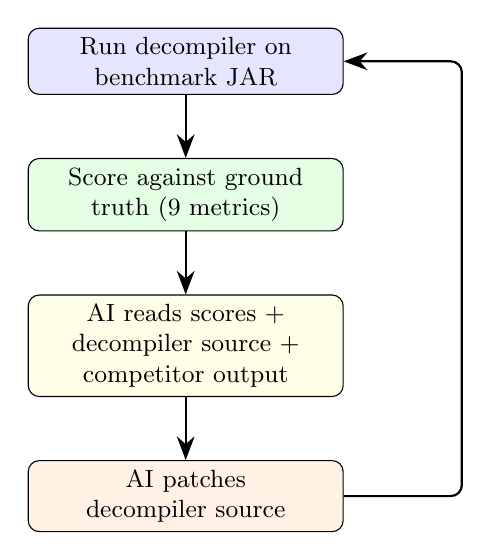
\begin{tikzpicture}[
    box/.style={draw, rounded corners, minimum width=4cm, minimum height=0.8cm, align=center, font=\small},
    arr/.style={-{Stealth[length=3mm]}, thick},
    node distance=0.8cm
]
\node[box, fill=blue!10] (run) {Run decompiler on\\benchmark JAR};
\node[box, fill=green!10, below=of run] (score) {Score against ground\\truth (9 metrics)};
\node[box, fill=yellow!10, below=of score] (read) {AI reads scores +\\decompiler source +\\competitor output};
\node[box, fill=orange!10, below=of read] (patch) {AI patches\\decompiler source};

\draw[arr] (run) -- (score);
\draw[arr] (score) -- (read);
\draw[arr] (read) -- (patch);
\draw[arr, rounded corners] (patch.east) -- ++(1.5,0) |- (run.east);
\end{tikzpicture}
\caption{Recursive self-improvement loop. The AI agent has full read/write access to the decompiler source code.}
\label{fig:loop}
\end{figure}

\begin{enumerate}
    \item \textbf{Benchmark execution}: The decompiler processes all classes in the benchmark JAR. Competing decompilers (CFR, Procyon, Vineflower, FernFlower) process the same inputs.
    \item \textbf{Scoring}: All outputs are normalized and scored against original source using the 9-metric composite.
    \item \textbf{AI analysis}: Claude Code reads the per-file scores, identifies weak files, reads the relevant decompiler source code, and reads competitor output for comparison.
    \item \textbf{Patching}: Claude Code proposes and applies modifications to the decompiler source code---new pattern recognizers, improved optimization passes, bug fixes.
    \item \textbf{Iteration}: Return to step 1.
\end{enumerate}

\subsection{AI Agent Capabilities}

The AI agent (Claude Code, powered by Claude Opus) has access to:
\begin{itemize}
    \item Full read/write access to all TypeScript source files
    \item Shell execution for building and running tests (\texttt{bun vitest})
    \item Benchmark execution and score inspection
    \item Competing decompilers' output files
    \item The competing decompilers' own source code (where available)
\end{itemize}

\subsection{Observed Modifications}

Across iterations, the AI agent made the following categories of modifications:

\textbf{Control flow improvements}: Identified cases where the linearizer was unnecessarily falling back to state-machine emission and added pattern recognizers for specific CFG topologies.

\textbf{Optimization enhancements}: Strengthened constant folding to handle additional expression types and expanded the conditions under which folding is applied.

\textbf{Competitor-inspired heuristics}: After observing that CFR cleanly decompiled switch statements where all cases terminate with \texttt{return}, added a similar heuristic to the switch decompiler.

\textbf{Bug fixes}: Corrected redundant cast emission in the expression-to-source converter and fixed edge cases in phi expression handling.

\subsection{Convergence Behavior}

Improvements are front-loaded: the largest score gains occur in the first 3--5 iterations, with diminishing returns thereafter. The agent occasionally proposes changes that improve scores on some files while regressing others; the per-file statistical breakdown enables detection and rollback of such changes.

%% ============================================================
\section{AI Post-Processor}
\label{sec:postprocessor}

Independently of the self-improvement loop, the \texttt{java-decompiler-ts-ai} package provides an inference-time cleanup agent. This is architecturally distinct from the loop: the loop modifies the decompiler's \emph{source code} (persistent), while the post-processor modifies the decompiler's \emph{output} (per-invocation).

\subsection{Architecture}

The \texttt{AIPostProcessor} executes a four-stage pipeline:

\begin{enumerate}
    \item \textbf{Workspace creation}: Decompiled sources are written to a temporary directory.
    \item \textbf{Agent initialization}: An AI session is created with a constrained system prompt and an MCP (Model Context Protocol) server exposing a \texttt{file\_done} tool for progress tracking.
    \item \textbf{Sequential processing}: The agent reads, edits, and writes back each file sequentially, calling \texttt{file\_done} after each.
    \item \textbf{Results}: Modified sources are read back and the workspace is cleaned up.
\end{enumerate}

\subsection{Constraints}

The system prompt enforces strict behavioral boundaries:
\begin{itemize}
    \item Preserve all logical behavior (control flow, signatures, types, observable semantics)
    \item Fix formatting (4-space indentation, consistent braces)
    \item Rename only auto-generated locals (\texttt{var1}, \texttt{v0}, \texttt{i\$})
    \item Fix obvious decompiler artifacts (unnecessary casts, broken string concatenation)
    \item Do \emph{not} add comments, documentation, annotations, methods, fields, or classes
\end{itemize}

This separation of concerns allows measuring the marginal contribution of each system: the decompiler's structural quality (loop) versus cosmetic cleanup (post-processor).

%% ============================================================
\section{Experimental Results}
\label{sec:results}

\subsection{Benchmark Configuration}

We evaluate on a benchmark JAR containing 47 Java source files spanning a range of language features: basic control flow, exception handling, generics, lambdas, switch expressions, inner classes, and enum types.

\subsection{Comparative Results}

Table~\ref{tab:results} presents the composite similarity scores after iterative self-improvement.

\begin{table}[t]
\centering
\caption{Decompiler Composite Similarity Scores}
\label{tab:results}
\begin{tabular}{@{}clcc@{}}
\toprule
\textbf{Rank} & \textbf{Decompiler} & \textbf{Composite} & \textbf{Match Rate} \\
\midrule
1 & Vineflower & 0.9360 & 47/47 (100\%) \\
2 & Procyon & 0.9010 & 47/47 (100\%) \\
3 & CFR & 0.8760 & 47/47 (100\%) \\
4 & BlackSwan (ours) & 0.8693 & 47/47 (100\%) \\
\bottomrule
\end{tabular}
\end{table}

BlackSwan achieves a composite score of 0.8693, within 0.7\% of CFR (0.8760) and within 7.1\% of Vineflower (0.9360). Notably:

\begin{itemize}
    \item BlackSwan successfully decompiles all 47 files (100\% match rate), matching the established tools.
    \item The gap to CFR---a decompiler with over a decade of development---is less than 1 percentage point.
    \item The entire BlackSwan codebase was developed in approximately two weeks, with Claude Code performing the majority of implementation work.
\end{itemize}

\subsection{Development Efficiency}

The ASM port was completed in approximately 4--5 hours of continuous Claude Code (Opus) execution, with convergence defined as passing round-trip byte-equality tests on three reference JARs. The IR, analysis, and decompiler layers were built iteratively with Claude Code against test cases.

%% ============================================================
\section{Applications to Automated Deobfuscation}
\label{sec:deobfuscation}

The recursive self-improvement loop has direct implications for reversing obfuscated software. We outline three application scenarios.

\subsection{Obfuscator-Specialized Decompilers}

Given:
\begin{itemize}
    \item A set of paired samples (original source, obfuscated output) from a known obfuscator
    \item Optionally, the obfuscator's source code
\end{itemize}

The loop can be configured with the obfuscated-vs-original pairs as the benchmark. The AI agent, with access to the obfuscator implementation, can write targeted deobfuscation passes that reverse specific transforms: string decryption, control flow de-flattening, reflection proxy removal, etc.

The resulting decompiler variant is \emph{specialized} for that obfuscator---not a general-purpose tool handling obfuscation heuristically, but a targeted pipeline with transform-specific inverse operations.

\subsection{Malware Family Analysis}

When multiple malware samples share an obfuscation toolchain, the loop can specialize against the common obfuscator. New samples from the same family would be decompiled by the specialized variant, producing substantially cleaner output than general-purpose decompilers.

\subsection{Obfuscator Fingerprinting}

Composite similarity scores produced by obfuscator-specialized decompiler variants can serve as a fingerprint. A sample's relative score across multiple specialized variants indicates which obfuscation tool was applied, enabling automated attribution without manual reverse engineering.

%% ============================================================
\section{Discussion}
\label{sec:discussion}

\subsection{Limitations}

\textbf{Exception handling}: The structured control flow decompiler currently rejects methods containing exception handlers, falling back to state-machine emission. This is a significant limitation for real-world code and a priority target for future loop iterations.

\textbf{Benchmark coverage}: Our 47-file benchmark, while spanning diverse language features, is limited in scale. Evaluation on larger, real-world codebases is needed.

\textbf{Loop convergence}: Improvements diminish after approximately 5 iterations. Whether this reflects fundamental limits of the current architecture or the AI agent's reasoning capacity is an open question.

\textbf{Regression risk}: The agent occasionally proposes changes that improve some files while degrading others. Human oversight is currently required to accept or reject proposed patches.

\subsection{Persistent vs.\ Inference-Time Improvement}

A key distinction of our approach is that improvements are \emph{persistent}---they are source code modifications committed to the codebase and applied to all future inputs. This contrasts with inference-time approaches (including our own AI post-processor) where each invocation incurs compute cost and may produce inconsistent results. The loop amortizes AI compute over all future decompilation runs.

\subsection{Language Choice as Architecture}

The decision to implement in TypeScript rather than Java is not merely a tooling preference---it is an architectural choice that determines the effectiveness of the self-improvement loop. As AI coding agents improve at additional languages, this constraint may relax, but for current-generation models, TypeScript provides a meaningfully better substrate for AI-driven code modification.

%% ============================================================
\section{Conclusion}
\label{sec:conclusion}

We have presented BlackSwan, a Java decompiler that improves through recursive AI-driven modification of its own source code. The system demonstrates that closing the loop between an AI coding agent, a multi-metric benchmark, and an editable decompiler codebase produces measurable, persistent improvements in decompilation quality.

The key enablers are: (1) implementing the entire pipeline in a language amenable to AI editing, (2) designing a composite evaluation metric resistant to single-metric gaming, and (3) providing the AI agent with access to competing systems' output for differential analysis.

The resulting decompiler achieves competitive scores against tools with substantially longer development histories, and the loop architecture generalizes naturally to obfuscator-specialized decompilation---a direction with significant implications for malware analysis and software security.

All source code is available at \url{https://www.blackswan.sh}.

%% ============================================================

\bibliographystyle{IEEEtran}
\bibliography{references}

\end{document}
